%% ============================================================
%%  GNN-CB — How to Evaluate LLMs: With and Without Agent Mode
%%  Compile: pdfLaTeX — run twice
%% ============================================================
\documentclass[aspectratio=169,t,10pt]{beamer}

\usetheme{Madrid}
\usefonttheme{professionalfonts}

\usepackage[utf8]{inputenc}
\usepackage[T1]{fontenc}
\usepackage{amsmath,amssymb}
\usepackage{booktabs}
\usepackage{array}
\usepackage{colortbl}
\usepackage{xcolor}
\usepackage{graphicx}
\usepackage{listings}
\usepackage{tikz}
\usetikzlibrary{shapes.geometric,arrows,positioning,calc}

%% ─── Colours ─────────────────────────────────────────────────
\definecolor{GNNblue}{RGB}{21,101,192}
\definecolor{GNNteal}{RGB}{0,137,123}
\definecolor{GNNgreen}{RGB}{46,125,50}
\definecolor{GNNorange}{RGB}{230,81,0}
\definecolor{GNNred}{RGB}{183,28,28}
\definecolor{GNNpurple}{RGB}{103,58,183}
\definecolor{GNNgold}{RGB}{255,152,0}
\definecolor{GNNgray}{RGB}{80,80,80}

%% ─── Beamer colours ──────────────────────────────────────────
\setbeamercolor{palette primary}{bg=GNNblue,fg=white}
\setbeamercolor{palette secondary}{bg=GNNblue!80,fg=white}
\setbeamercolor{palette tertiary}{bg=GNNblue!60,fg=white}
\setbeamercolor{palette quaternary}{bg=GNNblue!40,fg=white}
\setbeamercolor{structure}{fg=GNNblue}
\setbeamercolor{frametitle}{bg=GNNblue,fg=white}
\setbeamercolor{block title}{bg=GNNblue!12,fg=GNNblue!80!black}
\setbeamercolor{block body}{bg=GNNblue!4}
\setbeamercolor{alertblock title}{bg=GNNred!15,fg=GNNred!80!black}
\setbeamercolor{alertblock body}{bg=GNNred!4}
\setbeamercolor{exampleblock title}{bg=GNNgreen!12,fg=GNNgreen!70!black}
\setbeamercolor{exampleblock body}{bg=GNNgreen!4}
\setbeamercolor{itemize item}{fg=GNNblue}
\setbeamercolor{itemize subitem}{fg=GNNteal}
\setbeamertemplate{itemize item}[circle]
\setbeamertemplate{itemize subitem}[triangle]
\setbeamertemplate{navigation symbols}{}
\setbeamertemplate{footline}[frame number]
\setbeamerfont{frametitle}{size=\normalsize,series=\bfseries}

%% ─── Listings ────────────────────────────────────────────────
\lstset{
  basicstyle=\scriptsize\ttfamily,
  keywordstyle=\color{GNNblue}\bfseries,
  commentstyle=\color{GNNteal},
  stringstyle=\color{GNNorange},
  numbers=none,
  frame=single,
  rulecolor=\color{GNNblue!25},
  backgroundcolor=\color{GNNblue!4},
  breaklines=true,
  xleftmargin=4pt, xrightmargin=4pt
}

%% ─── TikZ node styles ────────────────────────────────────────
\tikzstyle{pbox}  = [rectangle, rounded corners=3pt, draw, thick,
                     minimum width=2.0cm, minimum height=0.6cm,
                     align=center, inner sep=4pt, font=\small]
\tikzstyle{Binp}  = [pbox, fill=GNNblue!12,   draw=GNNblue]
\tikzstyle{Bprc}  = [pbox, fill=GNNteal!12,   draw=GNNteal]
\tikzstyle{Bllm}  = [pbox, fill=GNNpurple!14, draw=GNNpurple,
                     minimum width=2.2cm, minimum height=0.75cm]
\tikzstyle{Bout}  = [pbox, fill=GNNgreen!12,  draw=GNNgreen]
\tikzstyle{Berr}  = [pbox, fill=GNNred!12,    draw=GNNred, dashed]
\tikzstyle{Bgold} = [pbox, fill=GNNgold!20,   draw=GNNorange]
\tikzstyle{Bman}  = [pbox, fill=GNNorange!12, draw=GNNorange]

%% ─── Helpers ─────────────────────────────────────────────────
\newcommand{\yes}{\textcolor{GNNgreen}{\bfseries\checkmark}}
\newcommand{\no}{\textcolor{GNNred}{\bfseries\texttimes}}
\newcommand{\auto}{\textcolor{GNNgreen}{\bfseries Auto}}
\newcommand{\manual}{\textcolor{GNNorange}{\bfseries Manual}}

%% ─── Title metadata ──────────────────────────────────────────
\title[GNN-CB: LLM Evaluation Procedure]{%
  \textbf{Evaluating LLMs on GNN Competitions}\\[4pt]
  \normalsize With and Without Agent Mode}
\author[GNN-CB]{GNN Coding Benchmark}
\date{May 2026}
\institute[GNN-CB]{GNN Coding Benchmark}

%% =============================================================
\begin{document}
%% =============================================================

%% ── 1. Title ─────────────────────────────────────────────────
\begin{frame}[plain]
\titlepage
\end{frame}

%% =============================================================
\section{Overview}
%% =============================================================

%% ── 2. Overview ──────────────────────────────────────────────
\begin{frame}{What We Want to Do}

\begin{columns}[T]
\column{0.55\textwidth}
\begin{block}{Goal}
Evaluate how well an LLM can solve a GNN coding competition
\textbf{from scratch} — given only the competition repo.
\end{block}

\vspace{6pt}
\textbf{The LLM must:}
\begin{itemize}\itemsep=3pt
  \item Understand the task from the README
  \item Read and interpret the data files
  \item Write a complete GNN training script
  \item Generate \texttt{predictions.csv} for the test set
  \item Fix its own errors if the code crashes
\end{itemize}

\vspace{6pt}
\begin{alertblock}{Key constraint}
One frozen prompt template for all competitions.\\
No per-task hints. No examples. No human guidance.
\end{alertblock}

\column{0.42\textwidth}
\begin{block}{Two ways to run it}
\vspace{4pt}
\begin{center}
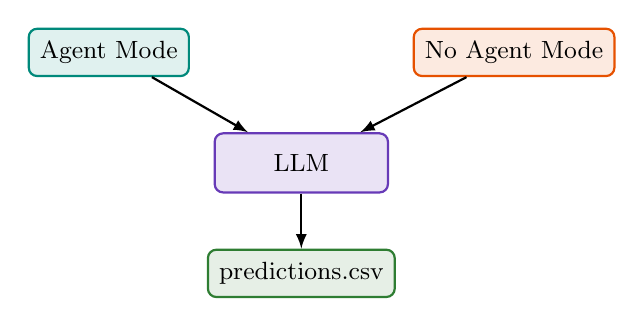
\begin{tikzpicture}[node distance=0.5cm, >=latex, thick]
  \node[Bllm] (llm) {LLM};
  \node[Bprc, above left=0.7cm and 0.3cm of llm]  (agent) {Agent Mode};
  \node[Bman, above right=0.7cm and 0.3cm of llm] (noagt) {No Agent Mode};
  \node[Bout, below=0.7cm of llm] (out) {predictions.csv};
  \draw[->] (agent) -- (llm);
  \draw[->] (noagt) -- (llm);
  \draw[->] (llm) -- (out);
\end{tikzpicture}
\end{center}
\vspace{4pt}
\textcolor{GNNgray}{\scriptsize Same output either way.\\Only the setup step differs.}
\end{block}
\end{columns}

\end{frame}

%% =============================================================
\section{Without Agent Mode}
%% =============================================================

%% ── 3. Without Agent Mode — Overview ─────────────────────────
\begin{frame}{Without Agent Mode --- The 3 Steps}

\begin{center}
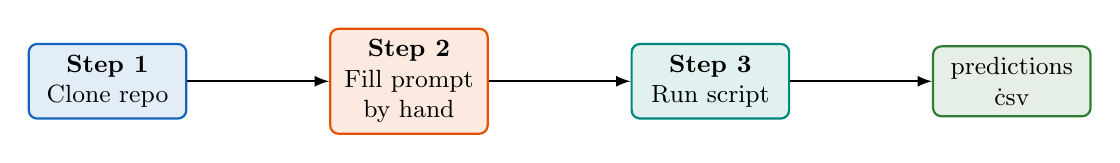
\begin{tikzpicture}[node distance=0.6cm and 1.8cm, >=latex, thick]

  \node[Binp] (s1) {\textbf{Step 1}\\Clone repo};
  \node[Bman, right=of s1] (s2) {\textbf{Step 2}\\Fill prompt\\by hand};
  \node[Bprc, right=of s2] (s3) {\textbf{Step 3}\\Run script};
  \node[Bout, right=of s3] (out) {predictions\\\.csv};

  \draw[->] (s1) -- (s2);
  \draw[->] (s2) -- (s3);
  \draw[->] (s3) -- (out);

\end{tikzpicture}
\end{center}

\vspace{4pt}

\begin{columns}[T]
\column{0.32\textwidth}
\begin{block}{\small Step 1 --- Clone}
\vspace{2pt}
{\scriptsize
\texttt{git clone <repo>}\\[2pt]
You now have all data files on your machine.
}
\end{block}

\column{0.32\textwidth}
\begin{alertblock}{\small Step 2 --- Fill Prompt}
\vspace{2pt}
{\scriptsize
Open \texttt{prompt.md}.\\
Paste 5 things from the repo:\\[2pt]
\textbullet\ README.md\\
\textbullet\ file tree (\texttt{find .})\\
\textbullet\ data shapes\\
\textbullet\ submission format\\
\textbullet\ requirements.txt\\[2pt]
Save as \texttt{prompt\_filled.md}
}
\end{alertblock}

\column{0.32\textwidth}
\begin{exampleblock}{\small Step 3 --- Run Script}
\vspace{2pt}
{\scriptsize
Open \texttt{GPT\_script.ipynb}.\\
Set your API key.\\
Run all cells.\\[2pt]
The script sends the prompt\\
to the LLM, runs the code,\\
and saves \texttt{predictions.csv}.
}
\end{exampleblock}
\end{columns}

\vspace{6pt}
\textcolor{GNNgray}{\scriptsize
Works with any LLM: GPT-4o, Llama, Mistral, Gemini, DeepSeek.
Only the API client changes. The loop is identical.}

\end{frame}

%% ── 4. Step 2 in detail: filling the prompt ──────────────────
\begin{frame}[fragile]{Without Agent Mode --- Step 2: Filling the Prompt}

\begin{columns}[T]
\column{0.48\textwidth}
\textbf{The frozen template has 5 slots:}

\vspace{4pt}
{\small
\begin{tabular}{@{}ll@{}}
\toprule
\textbf{Slot} & \textbf{Where to get it} \\
\midrule
\texttt{\{\{README\}\}}       & Paste \texttt{README.md} \\
\texttt{\{\{TREE\}\}}         & Run \texttt{find .\ -type f} \\
\texttt{\{\{DATA\_SHAPES\}\}} & Open each file, note sizes \\
\texttt{\{\{SUBMISSION\}\}}   & Paste submission section \\
\texttt{\{\{REQUIREMENTS\}\}} & Paste \texttt{requirements.txt} \\
\bottomrule
\end{tabular}
}

\vspace{8pt}
\begin{alertblock}{\small This is the only manual step}
{\scriptsize
You do it once per competition.\\
No coding needed — just copy and paste.\\
Save the result as \texttt{prompt\_filled.md}.
}
\end{alertblock}

\column{0.48\textwidth}
\textbf{What the filled prompt looks like:}

\vspace{4pt}
\begin{lstlisting}
## Competition README
<paste README.md here>

## Repository tree
<paste output of: find . -type f>

## Data sample
train_labels.csv: (3826, 2)
  node_id  label
  0        1
  1        0

## Submission format
predictions.csv with columns:
  node_id, pred_label

## Allowed libraries
<paste requirements.txt>

Produce <plan> then <code>.
\end{lstlisting}
\end{columns}

\end{frame}

%% ── 5. Step 3 in detail: the script loop ─────────────────────
\begin{frame}{Without Agent Mode --- Step 3: The Script Loop}

\begin{columns}[T]
\column{0.50\textwidth}

\begin{center}
\scalebox{0.88}{%
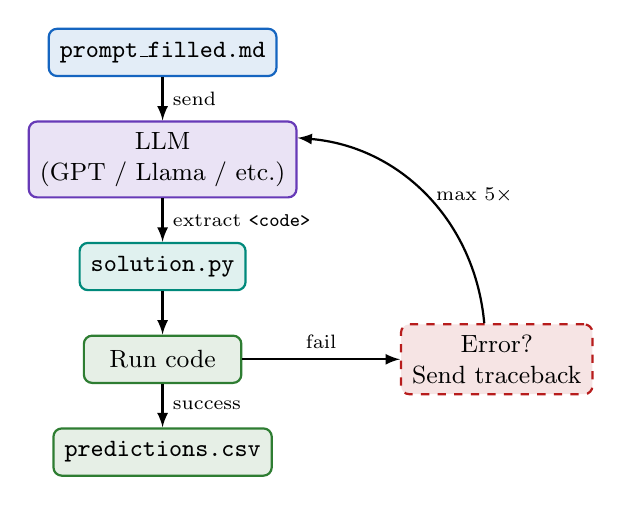
\begin{tikzpicture}[node distance=0.55cm, >=latex, thick]
  \node[Binp]  (pf)  {\texttt{prompt\_filled.md}};
  \node[Bllm,  below=of pf]  (llm)  {LLM\\(GPT / Llama / etc.)};
  \node[Bprc,  below=of llm] (sol)  {\texttt{solution.py}};
  \node[Bout,  below=of sol] (run)  {Run code};
  \node[Berr,  right=2.0cm of run]  (err)  {Error?\\Send traceback};
  \node[Bout,  below=of run] (out)  {\texttt{predictions.csv}};

  \draw[->] (pf)  -- node[right]{\scriptsize send} (llm);
  \draw[->] (llm) -- node[right]{\scriptsize extract \texttt{<code>}} (sol);
  \draw[->] (sol) -- (run);
  \draw[->] (run) -- node[right]{\scriptsize success} (out);
  \draw[->] (run) -- node[above]{\scriptsize fail} (err);
  \draw[->, bend right=40] (err) to node[right]{\scriptsize max 5$\times$} (llm);
\end{tikzpicture}
}
\end{center}

\column{0.46\textwidth}
\vspace{8pt}
\textbf{The script does 4 things:}
\begin{enumerate}\itemsep=4pt
  \item Sends \texttt{prompt\_filled.md} to the LLM
  \item Extracts the \texttt{<code>} block from the response
  \item Runs \texttt{python solution.py}
  \item If error: appends traceback and retries (max 5$\times$)
\end{enumerate}

\vspace{8pt}
\begin{block}{Works with any LLM}
{\scriptsize
\textbf{GPT-4o:} \texttt{from openai import OpenAI}\\
\textbf{Ollama:} same client, \texttt{base\_url=localhost}\\
\textbf{HuggingFace:} \texttt{transformers.pipeline(...)}\\[2pt]
Only 3 lines change. The loop is identical.
}
\end{block}
\end{columns}

\end{frame}

%% =============================================================
\section{With Agent Mode}
%% =============================================================

%% ── 6. With Agent Mode — Overview ────────────────────────────
\begin{frame}{With Agent Mode --- One Instruction Does Everything}

\begin{columns}[T]
\column{0.50\textwidth}

\begin{center}
\scalebox{0.88}{%
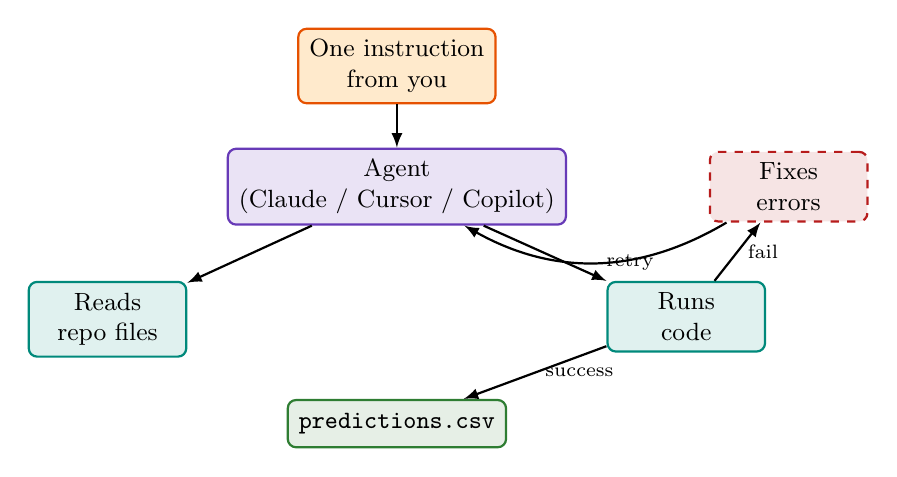
\begin{tikzpicture}[node distance=0.55cm, >=latex, thick]
  \node[Bgold] (inst) {One instruction\\from you};
  \node[Bllm,  below=of inst] (agt)  {Agent\\(Claude / Cursor / Copilot)};
  \node[Bprc,  below left=0.7cm and 0.5cm of agt]  (read) {Reads\\repo files};
  \node[Bprc,  below right=0.7cm and 0.5cm of agt] (run)  {Runs\\code};
  \node[Berr,  right=1.8cm of agt]  (fix)  {Fixes\\errors};
  \node[Bout,  below=2.2cm of agt]  (out)  {\texttt{predictions.csv}};

  \draw[->] (inst) -- (agt);
  \draw[->] (agt)  -- (read);
  \draw[->] (agt)  -- (run);
  \draw[->] (run)  -- node[right]{\scriptsize fail} (fix);
  \draw[->, bend left=30] (fix) to node[right]{\scriptsize retry} (agt);
  \draw[->] (run)  -- node[right]{\scriptsize success} (out);
\end{tikzpicture}
}
\end{center}

\column{0.46\textwidth}
\vspace{4pt}
\textbf{The agent does all of this automatically:}

\begin{itemize}\itemsep=3pt
  \item[\yes] Reads \texttt{README.md}
  \item[\yes] Gets repo file tree
  \item[\yes] Samples data files (shapes, head)
  \item[\yes] Reads \texttt{requirements.txt}
  \item[\yes] Fills the frozen prompt template
  \item[\yes] Writes \texttt{solution.py}
  \item[\yes] Runs \texttt{python solution.py}
  \item[\yes] Fixes errors (up to 5 times)
  \item[\yes] Saves all outputs
\end{itemize}

\vspace{4pt}
\textcolor{GNNgray}{\scriptsize You only set the repo path. Nothing else.}
\end{columns}

\end{frame}

%% ── 7. Which tools support agent mode ────────────────────────
\begin{frame}{With Agent Mode --- Supported Tools}

\vspace{4pt}
\begin{center}
{\small
\begin{tabular}{@{}llll@{}}
\toprule
\textbf{Tool} & \textbf{Agent Feature} & \textbf{LLM Backend} & \textbf{How to activate} \\
\midrule
Claude Code (CLI) & Agent mode (default)   & Claude        & \texttt{claude "instruction"} in terminal \\
Cursor            & Composer / Agent       & GPT / Claude  & \texttt{Ctrl+Shift+I} → Agent tab \\
VS Code Copilot   & Copilot Edits / Agent  & GPT           & Copilot Chat → switch to Agent \\
Windsurf          & Cascade                & Claude / GPT  & Open Cascade panel \\
Aider             & Default mode           & Any LLM       & \texttt{aider --message "..."} \\
OpenHands         & Full agent             & Any LLM       & Web UI or CLI \\
\bottomrule
\end{tabular}
}
\end{center}

\vspace{6pt}
\textbf{Example instruction (same for all tools):}

\vspace{2pt}
\begin{beamercolorbox}[rounded=true,shadow=false,wd=\textwidth]{block body}
{\scriptsize\ttfamily
Read the README, explore the data folder, then write and run solution.py\\
that trains a GNN and saves predictions.csv.\\
Use only the libraries in requirements.txt.\\
Follow the frozen prompt template at: llm\_real\_or\_fake/prompt.md
}
\end{beamercolorbox}

\end{frame}

%% =============================================================
\section{Comparison}
%% =============================================================

%% ── 8. Side-by-side comparison ───────────────────────────────
\begin{frame}{With vs.\ Without Agent Mode --- Side by Side}

\vspace{4pt}
\begin{center}
{\small
\setlength{\tabcolsep}{6pt}
\begin{tabular}{@{}lcc@{}}
\toprule
\textbf{Step} & \textbf{Agent Mode} & \textbf{No Agent Mode} \\
\midrule
Read README           & \auto  & \manual\ (paste into file) \\
Get repo file tree    & \auto  & \manual\ (run \texttt{find .}) \\
Sample data files     & \auto  & \manual\ (check shapes) \\
Fill prompt slots     & \auto  & \manual\ (save as \texttt{prompt\_filled.md}) \\
Write \texttt{solution.py}     & \auto  & \auto\ (via API script) \\
Run \texttt{solution.py}       & \auto  & \auto\ (via \texttt{subprocess}) \\
Fix errors (repair loop) & \auto & \auto\ (script sends traceback) \\
Save outputs          & \auto  & \auto\ (script copies files) \\
\midrule
\textbf{Manual steps for you} & \textbf{0} & \textbf{1} (fill prompt once) \\
\textbf{Works with GPT / open-source} & Depends on tool & \yes\ always \\
\textbf{Setup complexity} & Install agent tool & Python + API key only \\
\bottomrule
\end{tabular}
}
\end{center}

\vspace{6pt}
\begin{columns}[T]
\column{0.48\textwidth}
\begin{block}{Agent mode is best when\ldots}
{\scriptsize
You have Claude Code, Cursor, or Copilot already set up
and want zero manual work.
}
\end{block}
\column{0.48\textwidth}
\begin{exampleblock}{No agent mode is best when\ldots}
{\scriptsize
You want to use GPT, Llama, or any open-source LLM
with a simple Python script and no extra tools.
}
\end{exampleblock}
\end{columns}

\end{frame}

%% ── 9. Output produced either way ────────────────────────────
\begin{frame}{Output --- Same Either Way}

\begin{columns}[T]
\column{0.50\textwidth}

\textbf{Both approaches produce:}

\vspace{4pt}
\begin{beamercolorbox}[rounded=true,shadow=false,wd=\linewidth]{block body}
{\scriptsize\ttfamily
run\_<model>/\\
\quad plan.md \hfill\textcolor{GNNgray}{← LLM plan (architecture, protocol)}\\
\quad solution.py \hfill\textcolor{GNNgray}{← full GNN training script}\\
\quad execution\_log.txt \hfill\textcolor{GNNgray}{← stdout + stderr}\\
\quad predictions.csv \hfill\textcolor{GNNgray}{← test-set predictions}\\
\quad run\_summary.csv \hfill\textcolor{GNNgray}{← metrics}\\
}
\end{beamercolorbox}

\vspace{8pt}
\textbf{Example result (Real\_Or\_Fake, Claude):}

\vspace{4pt}
{\small
\begin{tabular}{@{}lr@{}}
\toprule
\textbf{Metric} & \textbf{Value} \\
\midrule
Validation F1       & 0.9768 \\
Validation Accuracy & 97.62\% \\
Threshold           & 0.53 \\
Epochs run          & 20 \\
Repair iterations   & 0 \\
\bottomrule
\end{tabular}
}

\column{0.46\textwidth}
\vspace{4pt}
\textbf{What we report for each (model, competition) pair:}

\begin{itemize}\itemsep=4pt
  \item Did the script run to completion?
  \item How many repair iterations were needed?
  \item Wall-clock time (CPU)
  \item Validation accuracy / F1
  \item Test-set predictions (for leaderboard)
\end{itemize}

\vspace{8pt}
\begin{alertblock}{Reproducibility}
{\scriptsize
The frozen prompt template is the only\\
prompt artifact released.\\[2pt]
Reproducing results requires only:\\
\textbullet\ the template\\
\textbullet\ the repo URL\\
\textbullet\ an API key
}
\end{alertblock}
\end{columns}

\end{frame}

%% ── 10. Summary ──────────────────────────────────────────────
\begin{frame}{Summary}

\begin{columns}[T]
\column{0.48\textwidth}
\begin{block}{The procedure in 3 steps}
\vspace{4pt}
{\small
\begin{enumerate}\itemsep=6pt
  \item \textbf{Clone} the competition repo
  \item \textbf{Prepare} the prompt\\
        \textcolor{GNNgreen}{\small Agent mode:} automatic\\
        \textcolor{GNNorange}{\small No agent mode:} paste 5 things manually
  \item \textbf{Run}\\
        \textcolor{GNNgreen}{\small Agent mode:} one instruction\\
        \textcolor{GNNorange}{\small No agent mode:} \texttt{GPT\_script.ipynb}
\end{enumerate}
}
\end{block}

\column{0.48\textwidth}
\begin{exampleblock}{Key points}
\vspace{4pt}
{\small
\begin{itemize}\itemsep=4pt
  \item Same frozen prompt template for both
  \item Same output: \texttt{predictions.csv}
  \item No agent mode works with \textbf{any LLM}\\
        (GPT, Llama, Mistral, Gemini\ldots)
  \item Agent mode works with Claude Code,\\
        Cursor, VS Code Copilot, Aider
  \item The repair loop is automatic in both
\end{itemize}
}
\end{exampleblock}
\end{columns}

\vspace{10pt}
\begin{center}
\textcolor{GNNblue}{\large\bfseries
The LLM receives the same information either way.\\[4pt]}
\textcolor{GNNgray}{\normalsize
Agent mode automates the preparation step. That is the only difference.}
\end{center}

\end{frame}

%% =============================================================
\end{document}
